
% !TeX root = ../treemap-taxonomy-ivapp2020.tex

%
{%
	%\pfinal
	%\scriptsize%
	\footnotesize
	\centering%
	%\newlength{\definitionswidth}%
	%\newlength{\definitionsoffset}%
	%\newlength{\definitionsimagesize}%
	%\newlength{\definitionsdescriptionsize}%
	\setlength{\definitionswidth}{\textwidth}%
	\setlength{\definitionsoffset}{13pt}%
	\setlength{\definitionsimagesize}{0.25\definitionswidth - 2\definitionsoffset}%
	\setlength{\definitionsdescriptionsize}{0.25\definitionswidth - 0.5\definitionsoffset}%
	\begin{tikzpicture}[]
	% Images
	\node[inner sep=0,outer sep=0] (space-filling) at (-1.5\definitionsimagesize - 3\definitionsoffset, 0.0) {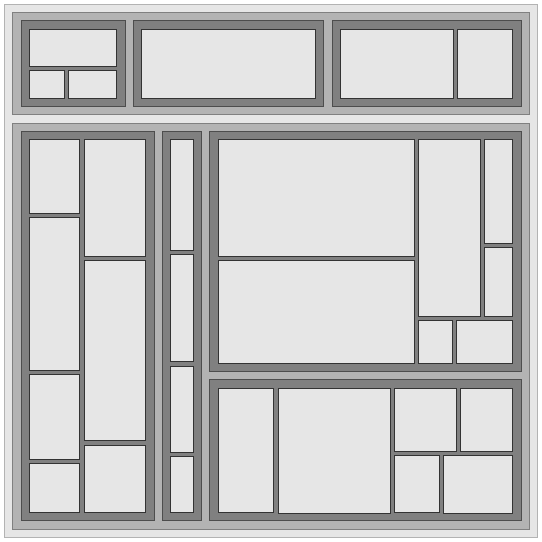
\includegraphics[width=\definitionsimagesize]{figures/treemap-cat-s}};
	\node[inner sep=0,outer sep=0] (containment) at (-0.5\definitionsimagesize + -1\definitionsoffset, 0.0) {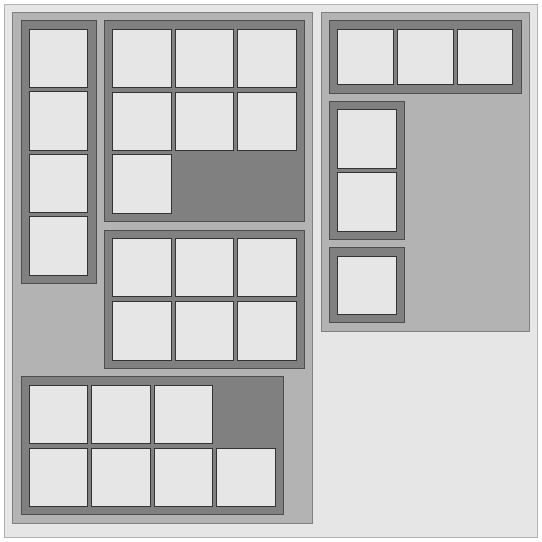
\includegraphics[width=\definitionsimagesize]{figures/treemap-cat-c}};
	\node[inner sep=0,outer sep=0] (implicit-edge) at (0.5\definitionsimagesize + 1\definitionsoffset, 0.0) {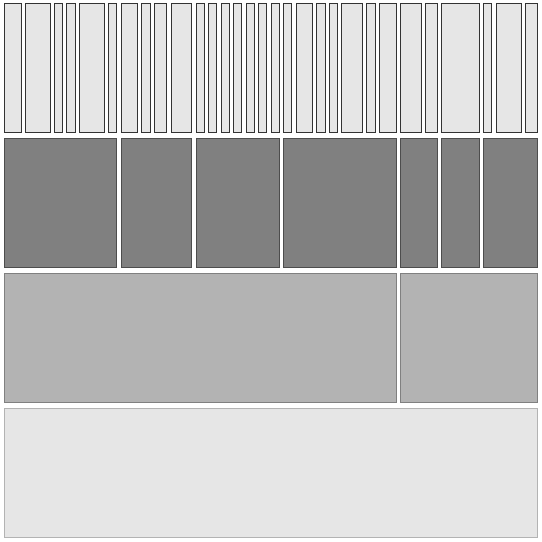
\includegraphics[width=\definitionsimagesize]{figures/treemap-cat-ie}};
	\node[inner sep=0,outer sep=0] (mapped-tree) at (1.5\definitionsimagesize + 3\definitionsoffset, 0.0) {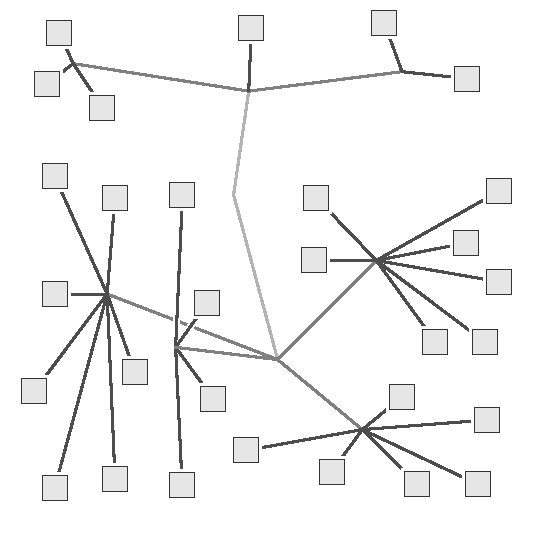
\includegraphics[width=\definitionsimagesize]{figures/treemap-cat-mt}};
	% Labels
	\node[above=0cm of space-filling] (tm0) {\Ts};
	\node[below=0cm of space-filling,text width=\definitionsdescriptionsize,align=center] (tm0-description) { Space-filling Treemap };
	\node[above=0cm of containment] (tm1) {\Tc};
	\node[below=0cm of containment,text width=\definitionsdescriptionsize,align=center] (tm1-description) { Containment Treemap };
	\node[above=0cm of implicit-edge] (tm2) {\Tie};
	\node[below=0cm of implicit-edge,text width=\definitionsdescriptionsize,align=center] (tm2-description) { Implicit Edge Representation Tree };
	\node[above=0cm of mapped-tree] (tm3) {\Tmt};
	\node[below=0cm of mapped-tree,text width=\definitionsdescriptionsize,align=center] (tm3-description) { Mapped Tree };
	\only<2-3|handout:1>{
		% Relations
		\draw[draw=none] (space-filling.east) -- (containment.west) node[pos=0.5] {\huge $\subset$};
		\draw[draw=none] (containment.east) -- (implicit-edge.west) node[pos=0.5] (splitting-subset) {\huge $\subset$};
		\draw[draw=none] (implicit-edge.east) -- (mapped-tree.west) node[pos=0.5] {\huge $\subset$};
	}
	\only<3|handout:1>{
		% Discriminator Line
		\draw[draw=none] (containment.center) -- (splitting-subset.center) node [pos=0.85] (discriminator-x) {};
		\draw[densely dotted,line width=0.75pt,shorten <= 5pt,shorten >= 5pt] (discriminator-x |- tm2.north) -- (discriminator-x |- tm2-description.south);
	}
	\end{tikzpicture}%
}%
%
